\documentclass[a4paper]{report}
\usepackage[utf8]{inputenc}
\usepackage[margin=1in]{geometry}
\usepackage[pagestyles]{titlesec}
\usepackage[hidelinks]{hyperref}
\usepackage{graphicx}
\renewcommand*{\arraystretch}{1.0}
\titleformat{\chapter}[display]{\normalfont\bfseries}{}{0pt}{\Huge}
\usepackage{titling}
\font\myfont=cmr12 at 35pt

\titlespacing*{\chapter}{0pt}{-30pt}{40pt}

\newcommand{\subtitle}[1]{%
  \posttitle{%
    \vspace*{1cm}
    \par\end{center}
    \begin{center}\large#1\end{center}
    \vspace*{1cm}}%
}

\renewcommand\contentsname{\vspace*{-70pt}} % Elimina la parola "Contents" dell'indice

\title{\myfont Smart Room}
\subtitle{\huge Progetto Numero \#3 del corso: \\ Embedded Systems and Internet of Things. \vspace*{0.5cm} \newline Sistema di automatizzazione della gestione di una Smart Room}
\author{\LARGE Nicola Montanari \vspace*{0.5cm} \\ \vspace*{0.5cm} \LARGE Nicola.Montanari14@studio.unibo.it \\ \LARGE 0000970119 \vspace*{1cm} \\ \LARGE Federico Muccioli \vspace*{0.5cm} \\ \vspace*{0.5cm} \LARGE federico.muccioli5@studio.unibo.it \\ \LARGE 0000971342 \vspace*{1.5cm}}

\date{Marzo 2023}

\begin{document}
\sloppy
\maketitle
\Large\tableofcontents
\newpage

\chapter{Room Mobile App}
\section{Descrizione}
La room mobile app consente di gestire la smart room tramite la tecnologia Bluetooth, comunicando direttamente con il room controller. \\
Questa applicazione è stata sviluppata in Java per Android e installata e testata su un dispositivo fisico dotato di sistema operativo Android 11. \\
L'app presenta due principali schermate o attività: la prima consente di gestire i dispositivi Bluetooth, mentre la seconda si occupa della connessione e dell'invio di messaggi.


\newpage
\vspace*{-1cm}
\section{Discovery Activity}
Per ottenere l'elenco dei dispositivi bluetooth è necessario richiedere l'attivazione del bluetooth del dispositivo e ottenere i permessi. \\
Una volta fatto ciò si otterrà una lista di dispositivi già accoppiati col device e la possibilità di effettuare una discovery per ottenere l'elenco dei dispositivi invece disponibili. \\
Eseguita una discovery i dispositivi disponibili invieranno un segnale intercettato poi dal BroadcastReceiver venendo poi aggiunti alla lista dei dispositivi disponibili.\\
Per quanto riguarda la UI è stato utilizzato un linear layout vertical che si adatta automaticamente alle dimensioni del device e presenta due ListView con i nomi dei dispositivi.\\
Alla ListView dei dispositivi disponibili viene impostato un Adapter che riceve come argomento una lista di stringhe con i nomi dei dispositivi. \\
Quando viene rilevato un nuovo dispositivo, la lista di stringhe viene aggiornata e viene richiamato il metodo notifyDataSetChanged() dell'Adapter, per aggiornare la ListView.\\
Per stabilire una connessione, è sufficiente selezionare il dispositivo desiderato da una delle ListView e si verrà reindirizzati alla seconda schermata dell'applicazione.\\

\begin{center}
   \fbox{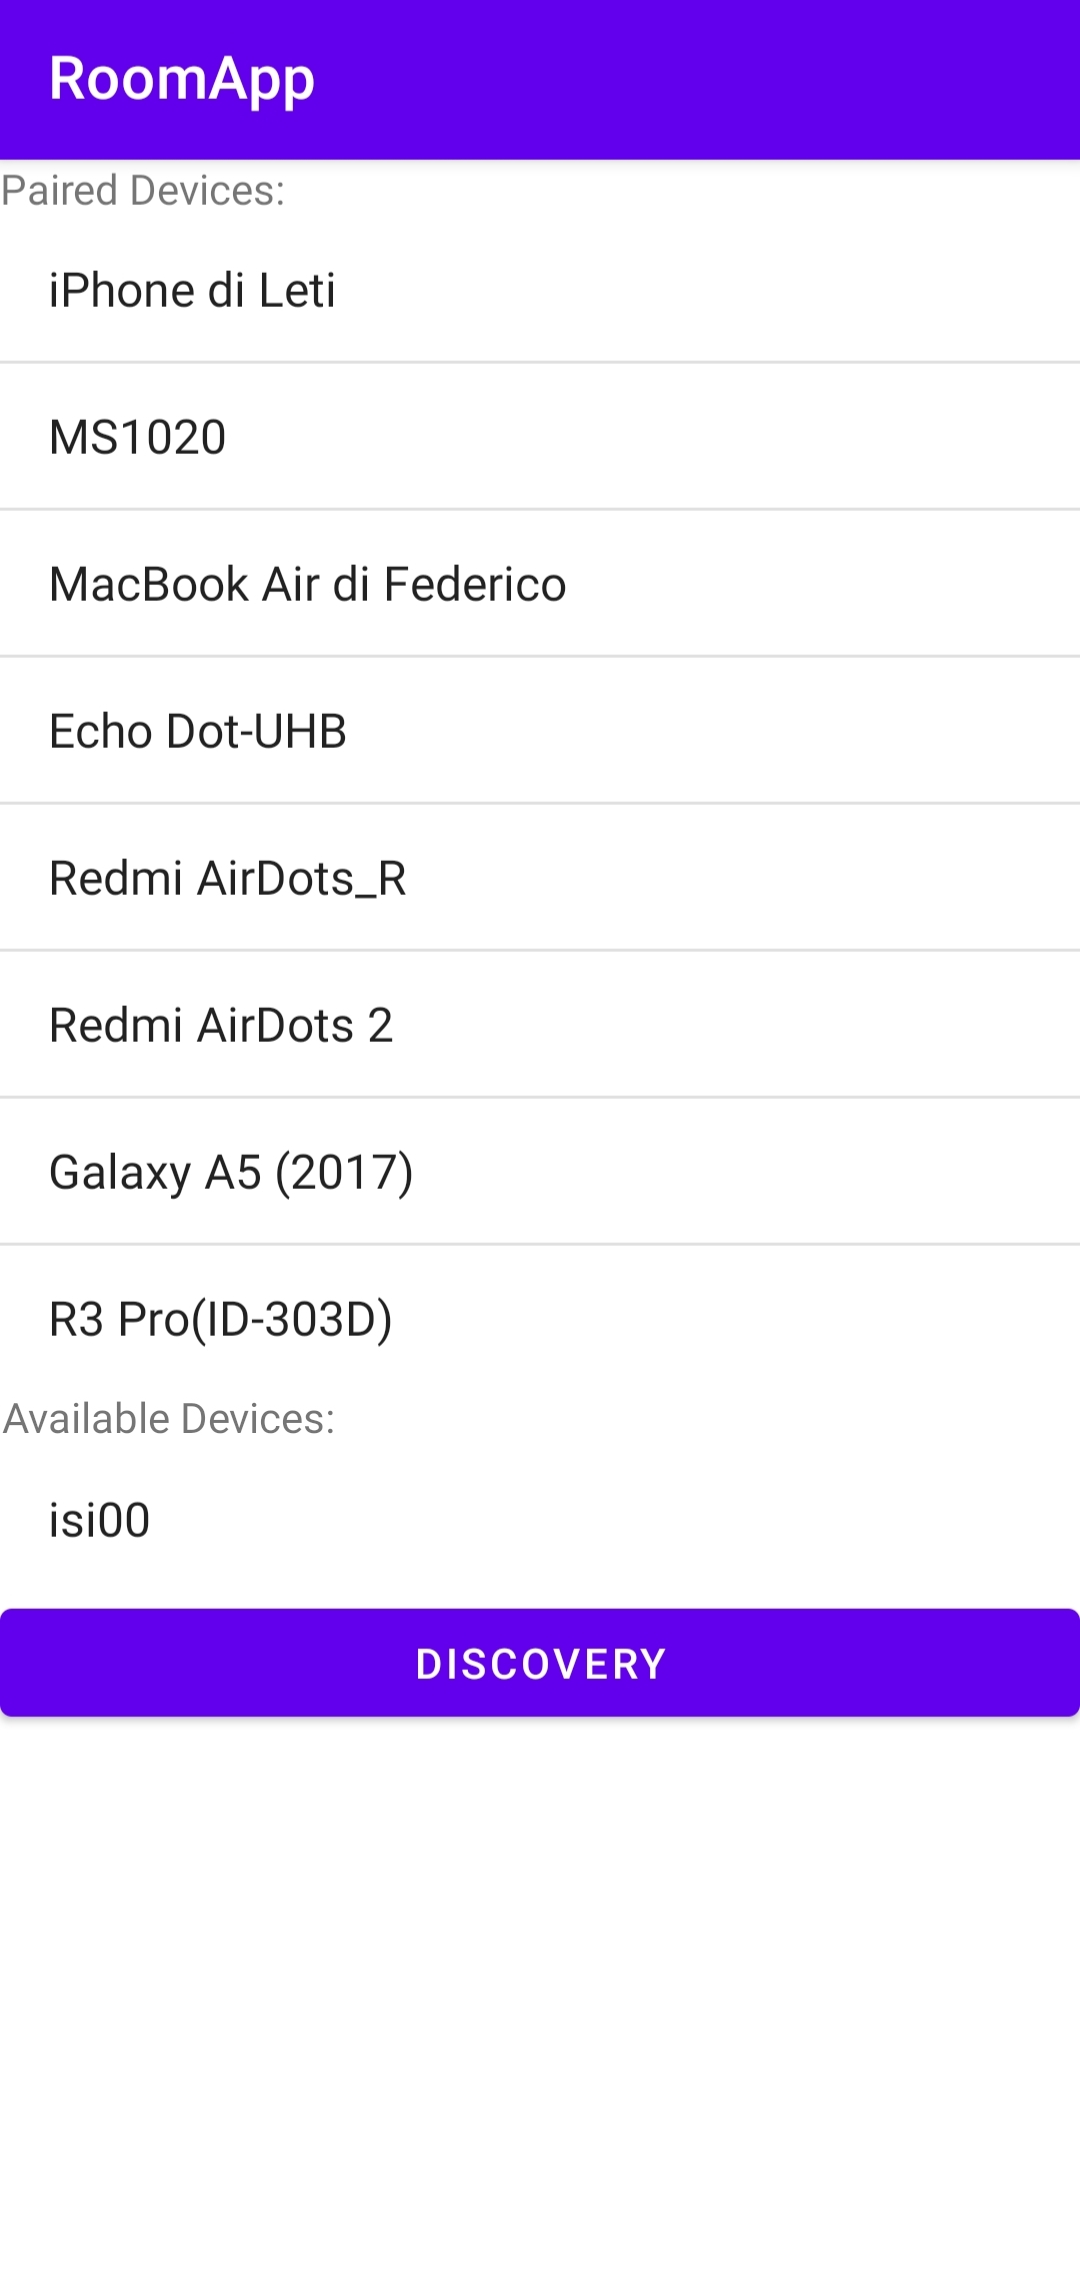
\includegraphics[scale=0.134]{images/AppDiscovery.png}}
\end{center}

\section{Controller Activity}
La schermata presenta una text view con il dispositivo al quale si sta tentando di connettersi, un bottone per accendere/spegnere la luce e uno slider per impostare le tapparelle da 0 a 100.
Come layout anche qui è stato utilizzato un LinearLayout questa volta orizzontale con impostazione gravity = center.
Finché la connessione con il dispositivo non sarà istanziata gli elementi dell'interfaccia saranno disabilitati e mostrati da una colorazione grigia.
Per la connessione sarà istanziato un nuovo thread così come per l'invio dei comandi e queste operazioni saranno delegate alla classe BluetoothRoomChannel.
Questa classe prenderà come parametri del costruttore il device al quale ci si vuole connettere, 
l'identificativo (UUID) e un handler definito con un unico metodo enable che permette in questo caso di attivare i componenti dell'attività. 
Una volta istanziato un BluetoothRoomChannel si avrà un socket tramite il quale richiamando il metodo run della classe verrà eseguita una connessione con un
nuovo thread ottenendo l'output stream e, se senza errori, verranno abilitati i componenti attraverso il metodo enable dell'handler. 
D'ora in poi per inviare messaggi basterà richiamare i relativi metodi di questa classe turnLight() e setRollerBlinds(percentage) che istanzieranno nuovi thread per la codifica e comunicazione.


\begin{center}
   \fbox{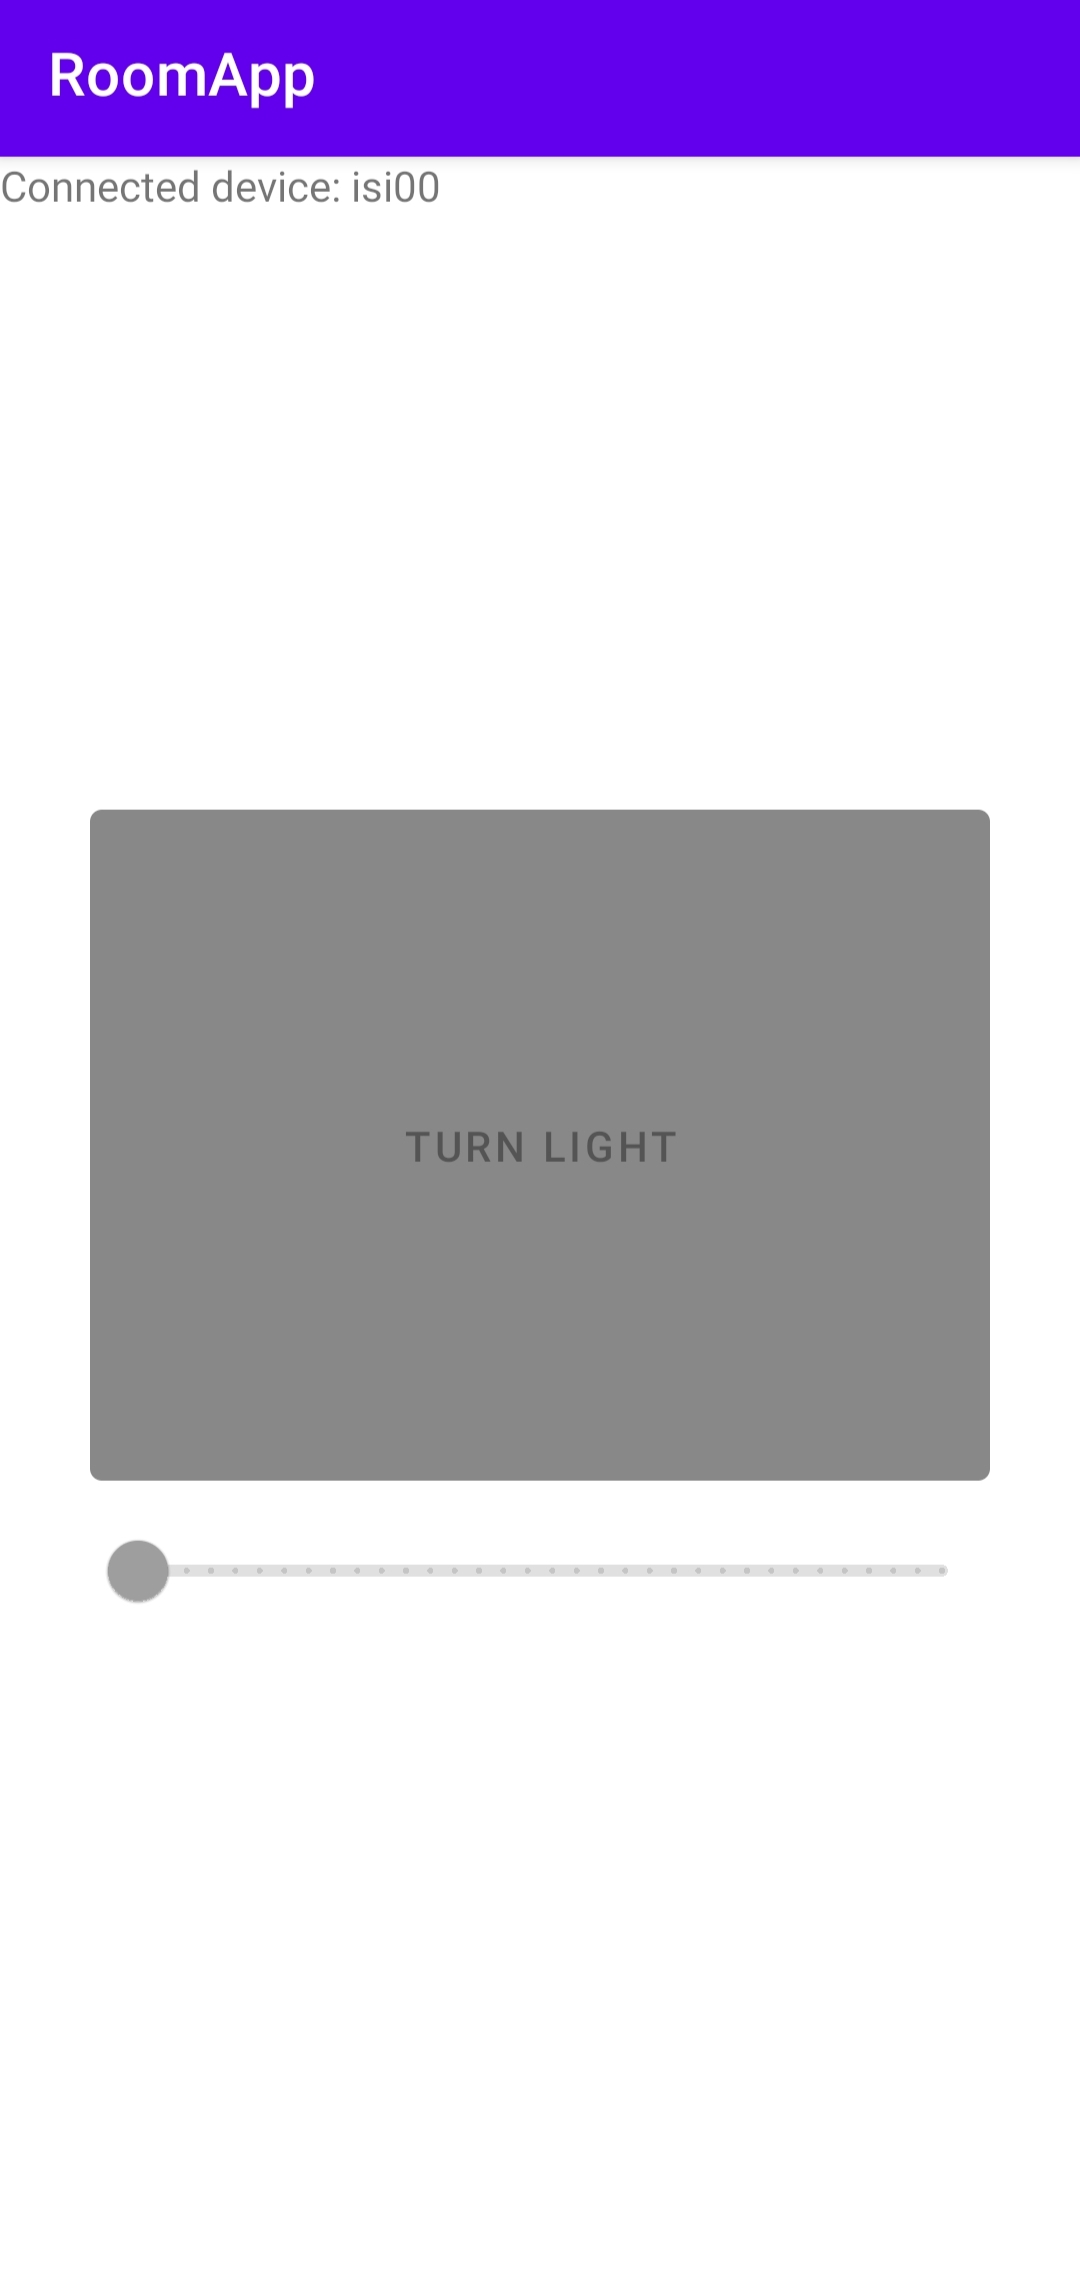
\includegraphics[scale=0.134]{images/AppControllerDisable.jpg}}
   \hspace{1cm}
   \fbox{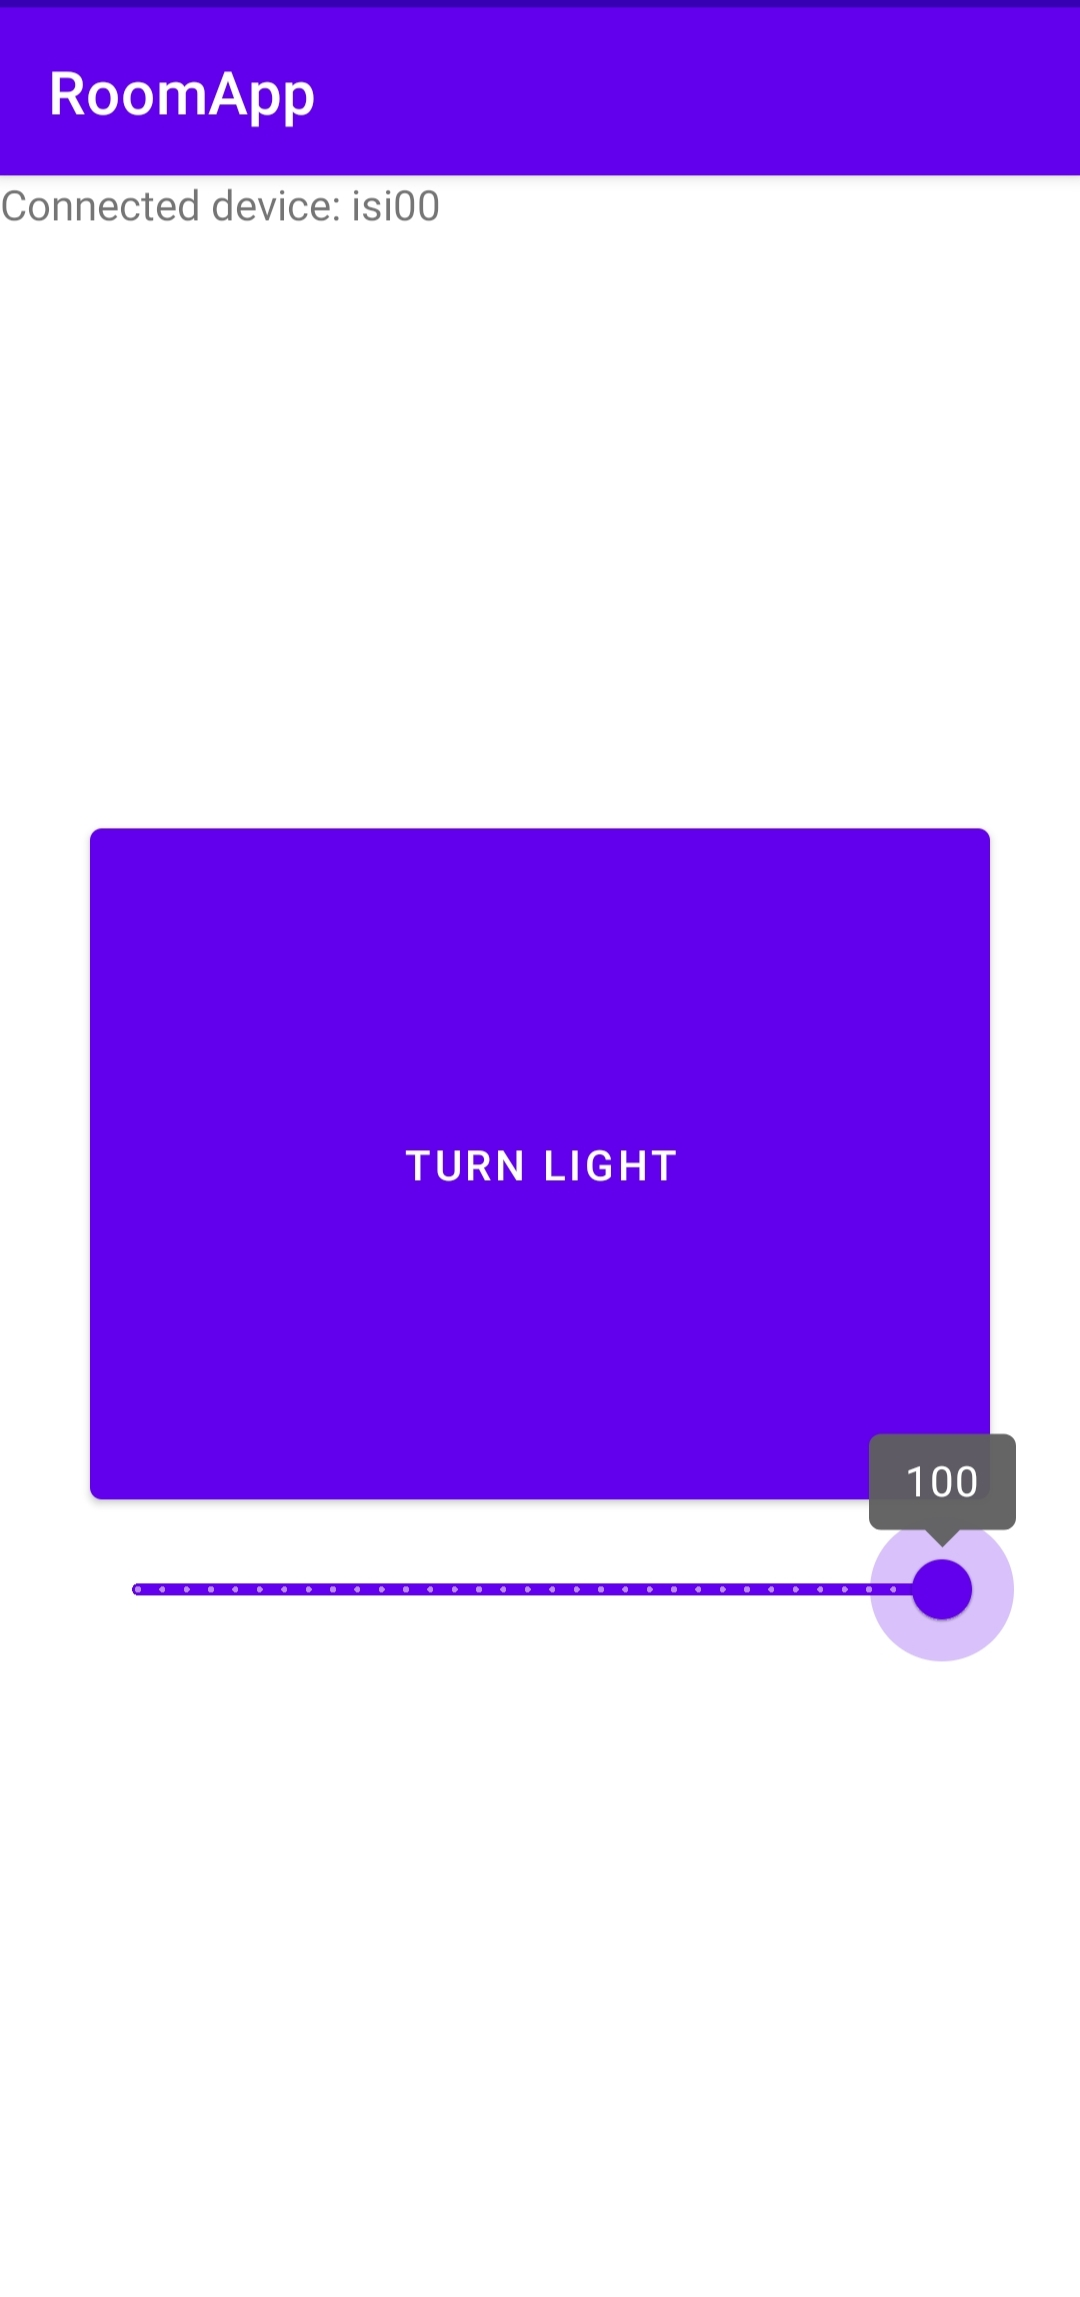
\includegraphics[scale=0.134]{images/AppControllerEnabled.jpg}}
\end{center}


\chapter{Room Controller}
\section{Descrizione}
Il sottosistema del room controller è composto dal microcontrollore Arduino, il quale è collegato tramite una porta seriale al room service e tramite il modulo bluetooth HC-06 alla room app.\\
Il microcontrollore Arduino riceve gli ordini di controllo e li esegue, pilotando la luce (simulata da un led) e le tapparelle (simulate da un servomotore).\\
Una volta completata l'esecuzione del comando, Arduino aggiorna il room service con lo stato attuale dei componenti controllati, fornendo così informazioni sulla loro posizione e stato di accensione o spegnimento.
\vspace{1cm}
\section{Schema Elettrico}

\begin{center}
   \fbox{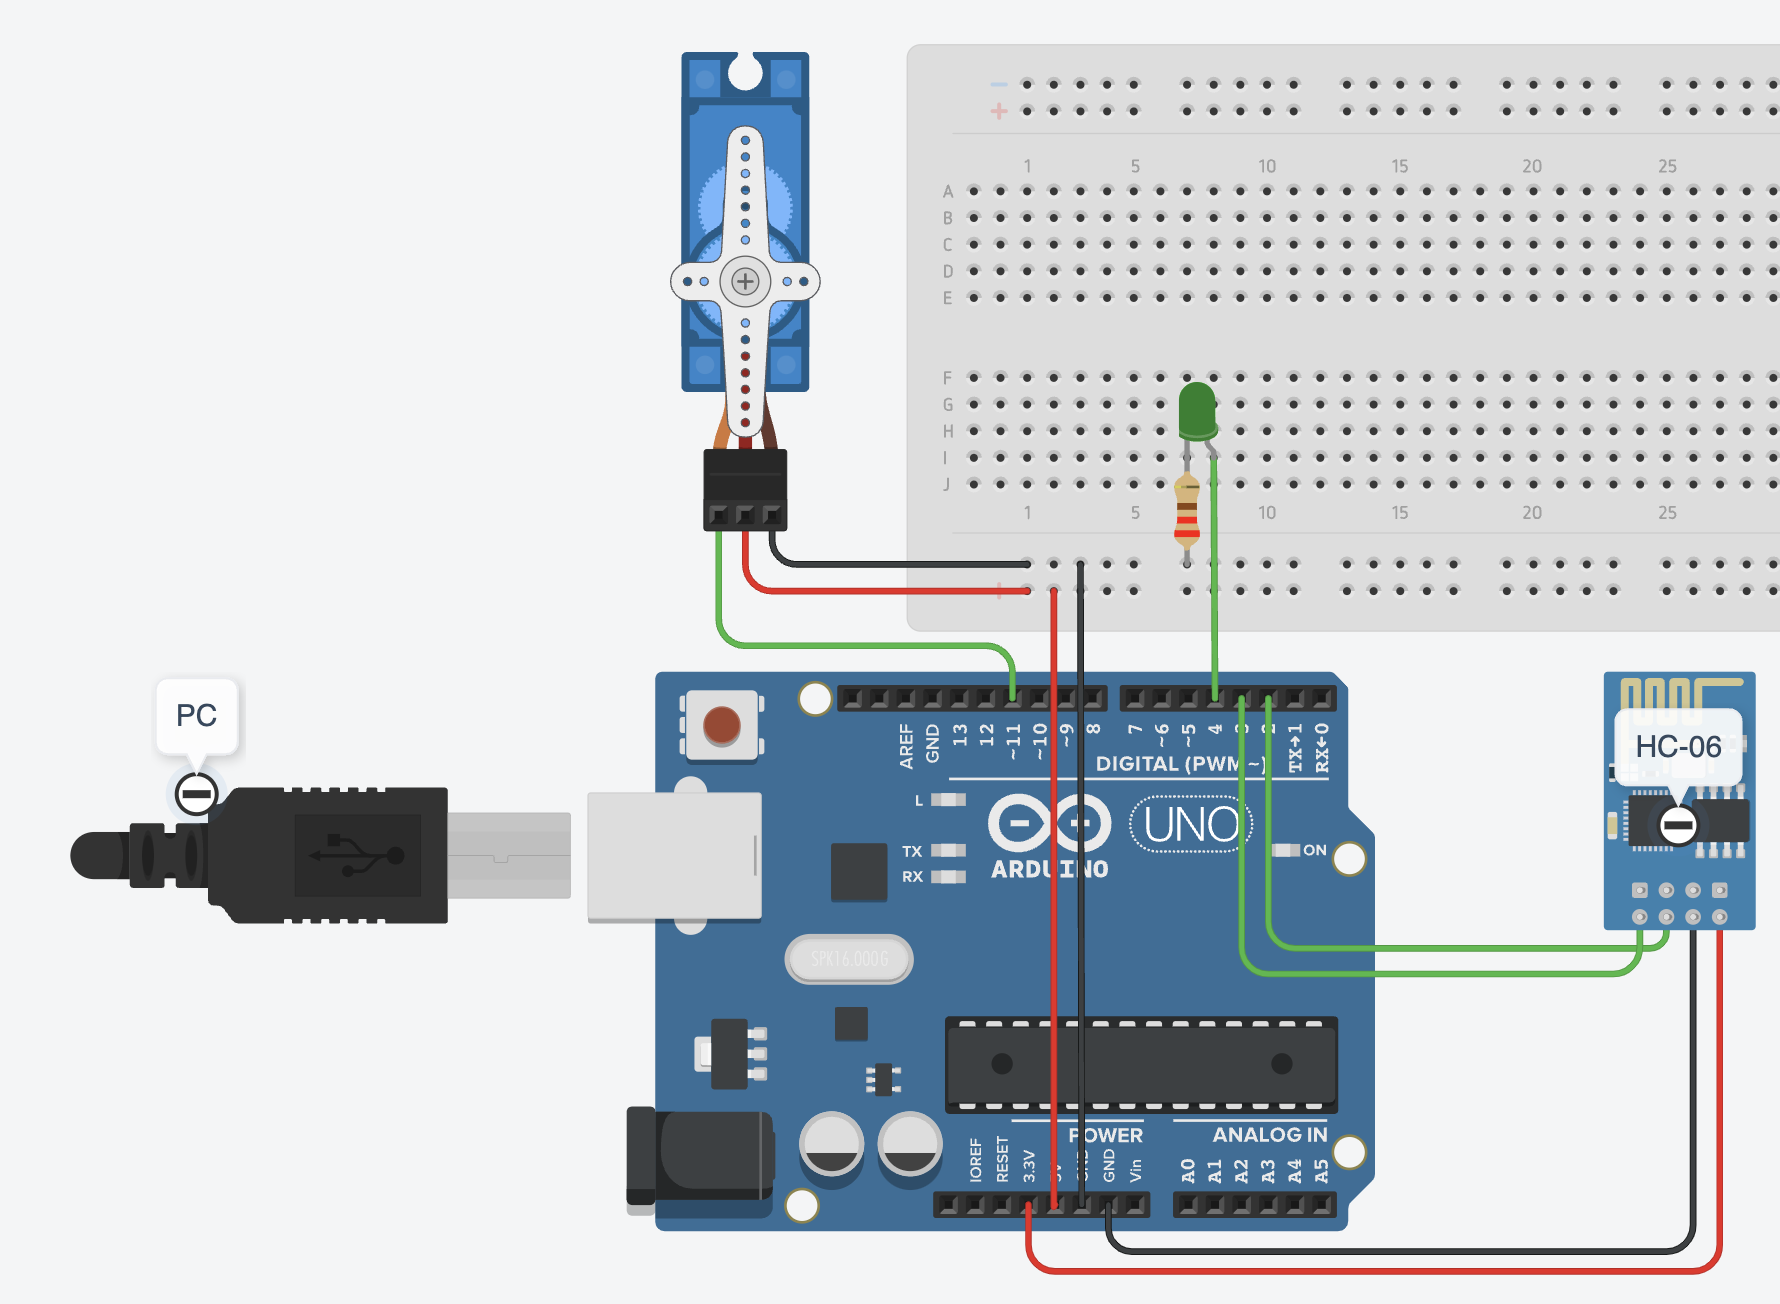
\includegraphics[scale=0.5]{images/ArduinoElectricalCircuit.png}}
\end{center}

\vspace{3cm}

\section{Scheduling e Task}
Nell'implementazione del sistema è stato definito un unico task che si trova costantemente nello
stesso stato, il quale verifica la ricezione di un messaggio, ne decodifica il contenuto, esegue il
comando sugli attuatori e invia una notifica al room service contenente i valori attuali dei
componenti controllati.\\
Per l'esecuzione del task è stato scelto un periodo di un secondo, in modo da garantire un'esecuzione abbastanza rapida dei comandi dal punto di vista dell'umano senza eccessiva reattività, limitando i consumi.\\
Inoltre, per limitare sempre i consumi del microcontrollore durante l'attesa dell'esecuzione del task, è stato impostato lo stato di sleep di Arduino con funzione IDLE, 
che consente comunque l'esecuzione dei timer necessari al funzionamento delle periferiche.\\
Al fine di garantire l'estendibilità del sistema in caso di integrazione di nuovi task, è stato implementato uno scheduler periodicizzato dal timer uno attraverso la libreria TimerOne.h.

\vspace{4cm}

\begin{center}
   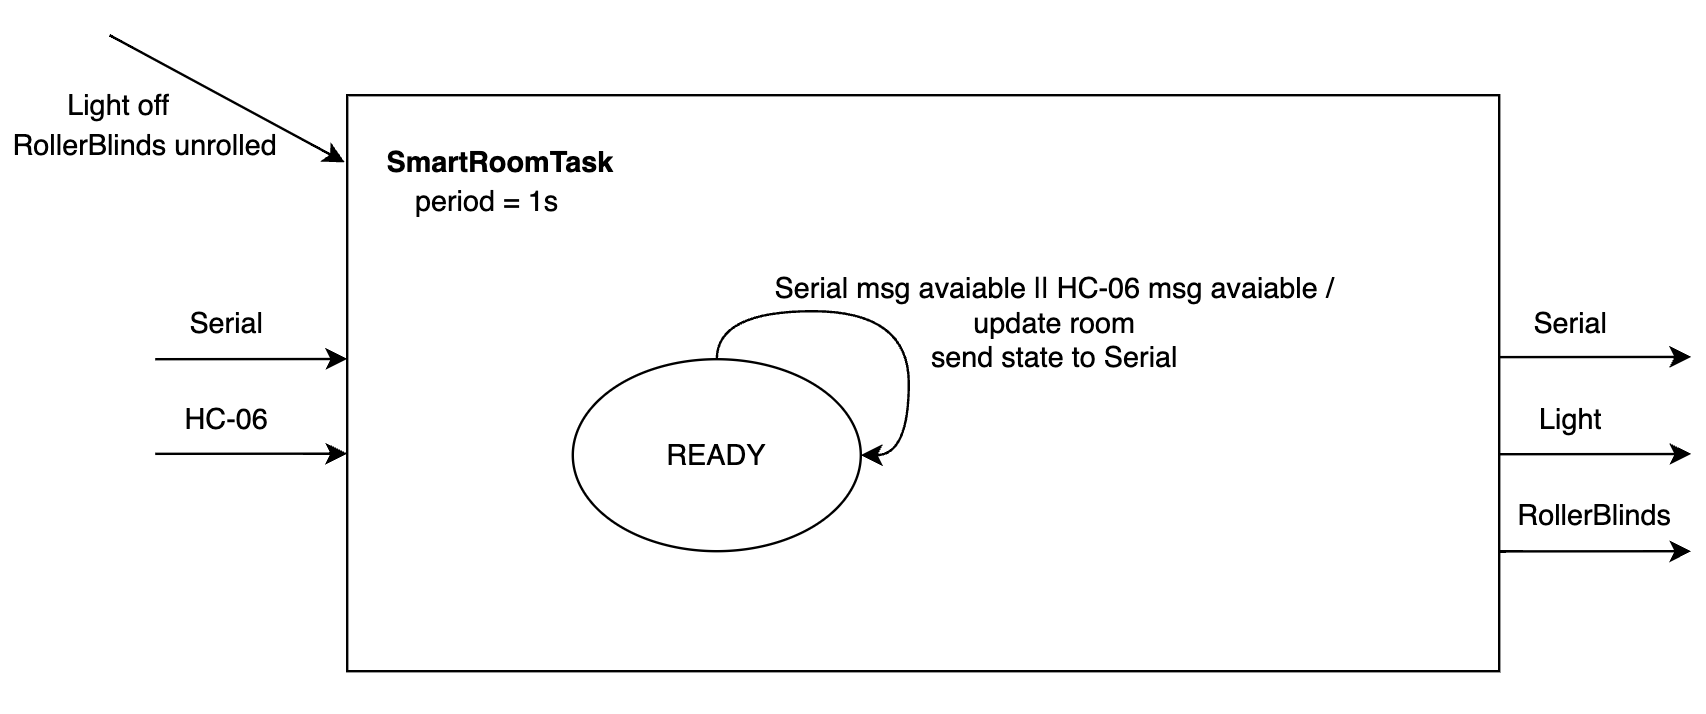
\includegraphics[scale=0.5]{images/ArduinoStateDiagram.png}
\end{center}

\newpage

\section{Comunicazione Bluetooth}
Poiché i pin 0 (RX) e 1 (TX) sono già utilizzati per la comunicazione seriale tra Arduino e il PC, il modulo Bluetooth è stato configurato come un dispositivo seriale tramite la libreria SoftwareSerial.h.\\
In particolare, la comunicazione è stata simulata tramite i pin 3 e 4.\\
Tuttavia, a causa della mancanza degli interrupt su questi pin, la verifica della ricezione di un messaggio avverrà solo tramite polling.




\section{Scelta Pin}
Poiché la libreria utilizzata per la comunicazione seriale sfrutta il timer1, è stata utilizzata un'altra libreria che utilizza il timer2 per gestire il servo motore.\\
Tuttavia, poiché il timer2 è anche utilizzato per la modulazione di larghezza di impulso (PWM) sui pin 3, 11, non è possibile utilizzare questa funzionalità quando il motore è attivo su questi pin. Per questo motivo, si è scelto di utilizzare i pin 3 e 11 per i dispositivi attuali che non richiedono la PWM, al fine di lasciare liberi questi pin per eventuali dispositivi futuri che ne necessitano.
\section{Gestione Comunicazione}
Poiché i comandi possono essere impartiti al room controller sia dalla room app che dal room service, è importante che il room service sia sempre a conoscenza dello stato attuale della stanza. Per questo motivo, ad ogni iterazione, Arduino deve inviare un messaggio di notifica al service contenente lo stato attuale dei componenti controllati, in modo da garantire che lo storico delle informazioni sia sempre corretto e aggiornato.\\
Poiché il room controller può ricevere messaggi da diversi sistemi contemporaneamente, è stato necessario adottare una soluzione che permettesse di gestire efficacemente l'arrivo di questi messaggi. 
Per questo motivo, è stata implementata una sorta di cache attraverso una lista FIFO con capacità massima di dieci messaggi, sufficiente per il periodo del task di un secondo.
\newpage

\section{Protocollo Comunicazione}
I messaggi con il room controller avvengono attraverso uno scambio di stringhe. La prima lettera della stringa definisce l'attuatore: "l" per light e "r" per le roller blinds.\\
I caratteri rimanenti rappresentano una cifra numerica, che nel caso delle tapparelle rappresenta la percentuale di apertura compresa tra 0 e 100, mentre nel caso della luce, 0 rappresenta la luce spenta, 1 rappresenta la luce accesa e 2 rappresenta il cambio di stato attuale.\\
Il room service riceverà un comando relativo a un singolo componente alla volta, mentre la notifica inviata dal room controller al room service avverrà tramite una singola stringa che conterrà i valori attuali dei vari componenti controllati, separati da una e commerciale "\&".





\chapter{Room Sensor-Board}
\section{Descrizione}
Il sottoprogetto Sensor-Board è composto da un microcontrollore ESP32 a cui sono stati collegati un sensore di luminosità, un PIR e un led. \\
L'ESP ha il compito di monitorare eventuali movimenti all'interno della stanza in cui è allocato, analizzare la luminosità circostante e di comunicare tramite protocollo MQTT le sue rilevazioni. \\ 
Ogni volta che il PIR rileverà dell'attività, verrà acceso il led presente nella configurazione e spento una volta terminata la rilevazione di movimento. \\
Il microcontrollore dovrà essere necessariamente collegato al WIFI affinchè possa inviare correttamente i messaggi tramite la rete.

\vspace{2cm}

\section{Schema Elettrico}


\begin{center}
   \fbox{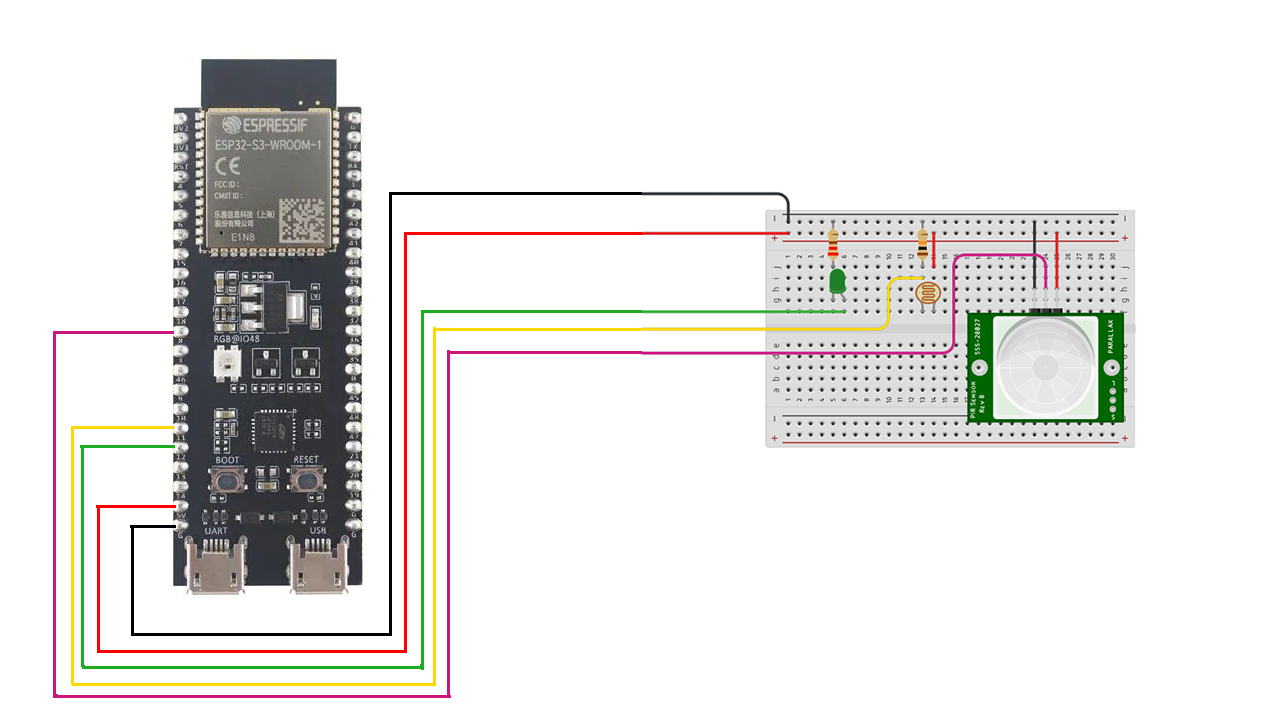
\includegraphics[scale=0.35]{images/ESP32ElectricalCircuit.png}}
\end{center}

\newpage
\section{Comportamento del Microcontrollore}
Il microcontrollore, appena viene alimentato, inizierà una procedura di connessione alla rete wifi, per poi assicurarsi di essere connesso al broker MQTT e al corretto Topic. \\
Una volta che queste impostazioni preliminari saranno state effettuate, verrà assegnata una task a un core dell'esp, che servirà a controllare all'infinito lo stato attuale della stanza e nel caso avvenga un cambiamento, inviare un messaggio.\\
Il core dell'ESP avrà il compito di assicurarsi che la connessione al broker MQTT risulti essere sempre attiva o nel caso avvenga una disconnessione, di riconnettersi. 

\vspace{2cm}
\begin{center}
   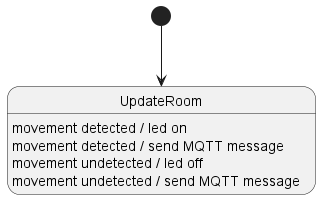
\includegraphics[scale=1]{images/sensor-board-state-scheme.png}
\end{center}

\newpage

\section{Comunicazione MQTT}
Per inviare messaggi, l'ESP32 utilizza il protocollo MQTT, sfruttando un broker presente online.\\
Sia quando viene rilevato del movimento sia quando il sensore non rileva piu movimento a seguito di un periodo di attività, il microcontrollore avrà il compito di inviare un messaggio; quest'ultimo non sarà altro che una stringa contenente l'eventuale inizio o fine dello stato di movimento e l'attuale luminosità della stanza, ottenuta tramite relativo sensore.\\
\vspace{1cm} \\
Esempio messaggio inviato tramite MQTT: \\
"MOTION\_DETECTED: ON \& LUMINOSITY: 400"
\vspace{1cm}
\section{Scelta Pin}
Siccome tutti i dispositivi necessari al progetto non presentano particolari vincoli in termine di pin, per il collegamento sono stati scelti dei pin generici presenti sulla scheda.



\chapter{Room Dashboard}
\vspace{1cm}
\section{Descrizione}
Lo scopo della Dashboard è quello di visualizzare lo stato delle luci e delle persiane nel corso del tempo e di poter controllare le luci e le persiane da remoto.
La Room Dashboard è stata implementata creando un sito web in HTML e gestendo la comunicazione HTTP con il Room Service tramite Javascript.
\vspace{2cm}
\section{Screenshot Applicazione}


\begin{center}
   \fbox{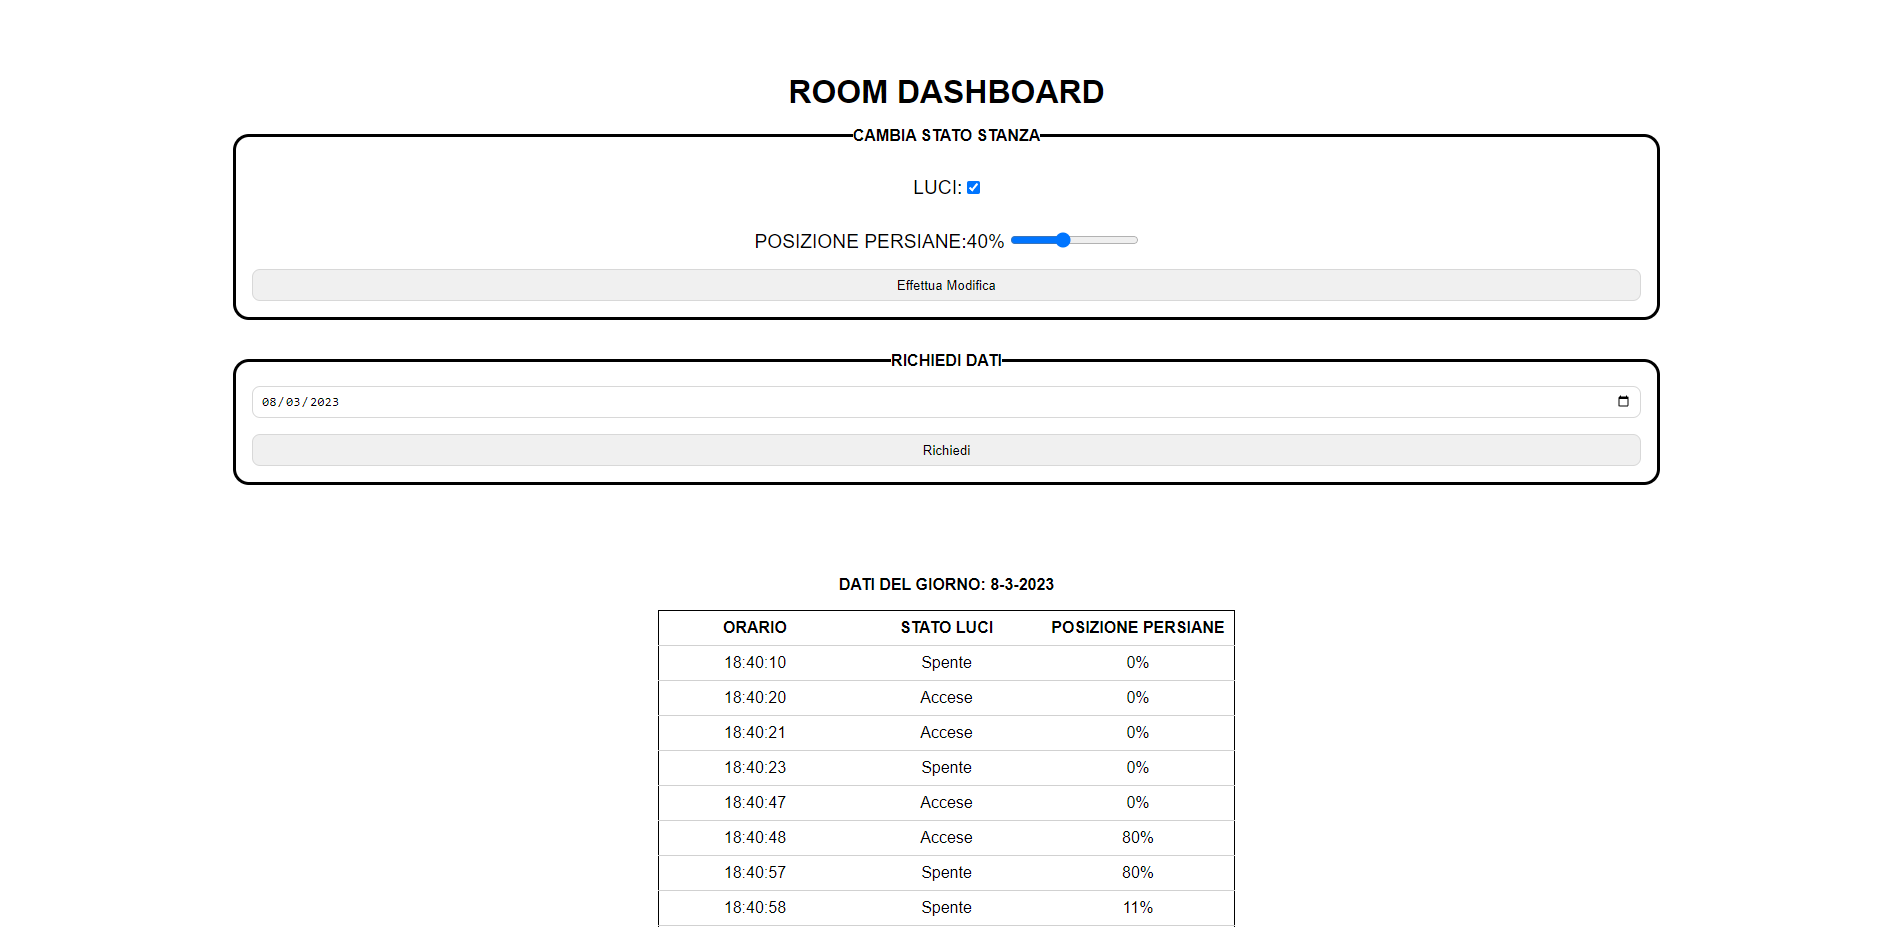
\includegraphics[scale=0.35]{images/ScreenDashboard.png}}
\end{center}

\newpage

\section{Struttura Sito Web}
Nella pagina web della dashboard sono presenti due form differenti, il primo serve ad effettuare modifiche alla stanza da remoto, mentre il secondo serve per richiedere i dati dello stato di una stanza di una giornata precisa.\\
In seguito a questi due form sarà presente una tabella contenente i vari dati se i dati richiesti sono effettivamente disponibili, o un messaggio di errore nel caso non lo siano.\\
Al caricamento della pagina verranno automaticamente richiesti i dati della giornata odierna.

\vspace{2cm}

\section{Comunicazione HTTP}
Per comunicare con il Room Service, il dashboard utilizza il protocollo HTTP inviando richieste GET o POST a seconda dell'esigenza dell'utente.\\
Nella casistica in cui un utente volesse cambiare lo stato della stanza da remoto, dovrà utilizzare il primo form citato precedentemente.\\
Una volta cliccato il tasto submit, verrà creata una stringa JSON con le informazioni estrapolate dalla pagina web, ovvero i valori dei due input presenti nel form: una checkbox per lo stato delle luci e uno slider per controllare la posizione delle persiane.\\
Questa stringa JSON verrà poi mandata tramite richiesta POST al Room Service, che invierà un messaggio di risposta con codice 200 se la ricezione sarà andata a buon fine.\\
Nella casistica invece che un utente voglia semplicemente visualizzare lo stato delle luci e delle persiane di un giorno preciso, dovrà compilare il secondo form presente nel sito inserendo la data cercata nell'apposito input field. \\
Dopo aver cliccato il relativo tasto submit, il dashboard invierà una richiesta GET al Room Service passando come parametro la data inserita.\\
Quest'ultimo, alla ricezione della data richiesta, andrà a cercare il relativo file JSON e invierà quest'ultimo sempre tramite protocollo HTTP inviandolo come risposta insieme al codice 200.\\
Se il file non risulta esistere, allora la risposta al dashboard avrà il codice 404 (Risorsa non trovata).




\chapter{Room Service}
\section{Descrizione}
Il room service si occupa di diverse mansioni, riceve input dai sensori della room sensor board che poi elabora per impartire comandi, comunica con il room controller per impartire comandi e ricevere lo stato della stanza ogni volta che varia e memorizza lo storico di tutte le variazioni della smart room che poi può essere richiesto dalla dashboard.\\
In pratica il room service è il sistema principale di gestione della smart room che comunica con gli altri sistemi utilizzando diverse tecnologie.

\vspace{2cm}
\section{Room Controller}
Il room service comunica con il room controller attraverso la seriale per impartire ordini e ricevere lo stato dei componenti della stanza. \\
La comunicazione avviene attraverso la classe RoomCommChannel che estende la classe SerialCommChannel che gestisce effettivamente la comunicazione seriale tramite la libreria jssc. \\
Il room service quando avrà bisogno di impartire ordini al room controller sfrutterà i metodi setLight e setRollerBlinds della classe RoomCommChannel che effettua una codifica dei messaggi in base al protocollo di stringhe descritto nel paragrafo riguardante il room controller e invierà i messaggi attraverso il metodo sendMsg della classe da cui ha esteso. \\
Quando invece Arduino comunicherà lo stato della stanza al programma Java, questo messaggio verrà intercettato, decodificato e verrà richiamato il metodo del controller che lo memorizzerà in un file Json.

\newpage

\section{Dashboard}
Per gestire le richieste in entrata dal Dashboard, nel Room service è stato sviluppato un HTTP Server che rimarrà permanentemente in ascolto nell'attesa di ricevere richieste GET o POST da un qualsiasi indirizzo.\\
Come già spiegato precedentemente nel Room-Dashboard, quando il Service riceverà richieste GET, utilizzerà il parametro inviato per ricercare il file JSON contenente i dati richiesti, per poi inviarlo come risposta al mittente della richiesta.\\
Nel caso il file ricercato non esista, verrà comunque inviata una risposta al client, ma con codice 404 (Risorsa non trovata).\\
Se invece la richiesta in entrata sarà di metodo POST, allora verranno estrapolati i dati allegati alla richiesta e verranno utilizzati per effettuare, tramite la classe "Controller", modifiche alla stanza (luci e/o persiane).

\vspace{2cm}
\section{Room Sensor-Board}
Affinchè il Service possa ricevere i messaggi MQTT inviati dall'ESP32 del Room Sensor-Board è stato necessario implementare un MQTT Agent all'interno del progetto.\\
Questa classe servirà a iscriversi allo stesso topic del microcontrollore, affinchè si possa gestire la ricezione dei messaggi e le operazioni necessarie in seguito alla ricezione a questi ultimi.\\
Infatti, quando un nuovo messaggio MQTT verrà postato nel topic condiviso, il Service avrà il compito di leggerlo e di estrapolare i dati al suo interno, ovvero lo stato del movimento e la luminosità della stanza (come spiegato precedentemente nel capitolo riguardante il Room Sensor-Board).\\
Una volta che i dati verranno estrapolati correttamente, saranno inviati alla classe "Controller" che deciderà poi se effettuare un cambiamento alla stanza o meno.\\
L'MQTT Agent viene avviato immediatamente al lancio dell'applicazione.\\


\end{document}
